\documentclass[a4paper,12pt]{article}

% Codificación y lenguaje
\usepackage[utf8]{inputenc}
\usepackage[T1]{fontenc}
\usepackage[spanish]{babel}
\usepackage[utf8]{inputenc}
\usepackage{caption}

% Paquetes esenciales
\usepackage{graphicx}
\usepackage{geometry}
\usepackage{datetime}
\usepackage{titlesec}
\usepackage{fancyhdr}
\usepackage{parskip}
\usepackage{array}
\usepackage{float}
\usepackage{placeins}
\usepackage{hyperref}
% Paquetes para código fuente
\usepackage{listings}
\usepackage{xcolor}
\usepackage{amsmath}  

% Configuración del estilo de listings para código Arduino
\lstdefinestyle{arduino}{
  language=C++,
  basicstyle=\ttfamily\footnotesize,
  keywordstyle=\color{blue},
  commentstyle=\color{gray},
  stringstyle=\color{red},
  numbers=left,
  numberstyle=\tiny,
  stepnumber=1,
  numbersep=5pt,
  backgroundcolor=\color{white},
  frame=single,
  breaklines=true,
  captionpos=b
}
\lstset{style=arduino}

% Márgenes del documento
\geometry{left=3cm, right=2.5cm, top=3cm, bottom=3cm}

\begin{document}

%\title{Trabajo Práctico 3: RISC-V Pipeline}
%\author{Agustín Trachta \and Agustín Pallardó}
%\date{\today}

%\begin{document}

%\maketitle
%\tableofcontents
%\newpage

\input{sections/00_caratula}
\newpage

\section{Introducción}

Un \textit{pipeline} es una técnica de diseño de procesadores que busca mejorar el rendimiento dividiendo la ejecución de cada instrucción en una serie de etapas secuenciales. De este modo, varias instrucciones pueden avanzar simultáneamente por distintas fases del procesamiento, lo que permite un mejor aprovechamiento de los recursos del sistema.

La arquitectura \textit{RISC-V}, basada en el paradigma \textit{Reduced Instruction Set Computer}, se destaca por su simplicidad, modularidad y carácter abierto. Estas características la convierten en una opción especialmente adecuada para estudiar la organización interna de un procesador y desarrollar implementaciones escalables, verificables y de complejidad controlada.

En este trabajo se presenta el diseño, la implementación y la validación de un procesador \textit{RISC-V} segmentado de cinco etapas sobre una FPGA Basys 3. El sistema desarrollado corresponde a un procesador de 32 bits organizado en las etapas \textit{Instruction Fetch} (IF), \textit{Instruction Decode} (ID), \textit{Execute} (EX), \textit{Memory Access} (MEM) y \textit{Write Back} (WB).

El objetivo principal es construir un \textit{pipeline} funcional capaz de ejecutar un subconjunto de instrucciones de la arquitectura RISC-V, garantizando el transporte correcto de datos y señales de control entre sus distintas etapas. Para ello, fue necesario diseñar tanto el camino de datos como la unidad de control, y resolver adecuadamente problemas asociados a dependencias de datos, riesgos de control y sincronización del flujo de ejecución.

Además, se incorporan mecanismos de observabilidad y depuración que permiten inspeccionar el estado interno del sistema durante su funcionamiento. Con este fin, se desarrolló una \textit{Debug Unit} que se comunica con el procesador mediante comandos enviados por UART, posibilitando la carga de programas en memoria, la ejecución paso a paso, la detención controlada y el volcado de registros, memoria y registros inter-etapa del \textit{pipeline}.

Este desarrollo integra módulos construidos en trabajos prácticos anteriores, en particular las unidades de ALU y UART (con leves modificaciones), incorporándolos dentro de una arquitectura más completa orientada no sólo a la ejecución de programas, sino también a su validación y depuración.

\newpage

\section{Objetivos}

\subsection{Objetivo general}

Implementar y validar el pipeline de un procesador RISC-V en una FPGA Basys 3.

\subsection{Objetivos específicos}

\begin{itemize}
    \item Implementar el pipeline del procesador RISC-V en Verilog, permitiendo la ejecución de instrucciones de manera correcta y eficiente.
    \item Desarrollar una Debug Unit que permita enviar y recibir información al procesador mediante el protocolo UART.
    \item Crear una interfaz para visualizar los datos e interactuar con la Debug Unit, utilizando CLI, GUI y/o TUI.
    \item Lograr que el procesador sea capaz de programarse y reprogramarse a través de comandos de UART.
    \item Garantizar que el clock no sea intervenido en ninguna parte del proyecto.
    \item Documentar decisiones tomadas en el diseño, justificando el razonamiento detrás de cada una.
    \item Creatividad al momento de mostrar los datos e interactuar con ellos (GUI, TUI, CLI).
\end{itemize}

\newpage

\section{Arquitectura del Procesador RISC-V}

\subsection{Formato de las Instrucciones}
La arquitectura RV32I utiliza instrucciones de 32 bits de longitud fija. Según el tipo de instrucción, esos 32 bits se organizan en distintos campos, como \texttt{opcode}, \texttt{rd}, \texttt{rs1}, \texttt{rs2}, \texttt{funct3}, \texttt{funct7} e inmediatos. Estos campos permiten identificar qué operación debe realizar el procesador, qué registros participan y si la instrucción requiere un valor inmediato.

Los formatos principales implementados en este procesador son: Tipo-R, Tipo-I, Tipo-S, Tipo-B, Tipo-U y Tipo-J.

\begin{table}[h]
\centering
\begin{tabular}{|c|p{10cm}|}
\hline
\textbf{Tipo} & \textbf{Campos} \\ \hline
R & \texttt{funct7 | rs2 | rs1 | funct3 | rd | opcode} \\ \hline
I & \texttt{imm[11:0] | rs1 | funct3 | rd | opcode} \\ \hline
S & \texttt{imm[11:5] | rs2 | rs1 | funct3 | imm[4:0] | opcode} \\ \hline
B & \texttt{imm[12|10:5] | rs2 | rs1 | funct3 | imm[4:1|11] | opcode} \\ \hline
U & \texttt{imm[31:12] | rd | opcode} \\ \hline
J & \texttt{imm[20|10:1|11|19:12] | rd | opcode} \\ \hline
\end{tabular}
\caption{Formatos principales de instrucciones en RV32I.}
\end{table}

Cada formato responde a una necesidad distinta dentro del conjunto de instrucciones:

\begin{itemize}
    \item \textbf{Tipo-R:} se utiliza para operaciones entre registros, como \texttt{add}, \texttt{sub}, \texttt{and}, \texttt{or}, \texttt{sll} o \texttt{slt}. En este caso, los campos \texttt{funct3} y \texttt{funct7} permiten distinguir la operación exacta.
    
    \item \textbf{Tipo-I:} se utiliza para instrucciones con inmediato, como \texttt{addi}, \texttt{andi}, \texttt{ori}, cargas desde memoria (\texttt{lb}, \texttt{lh}, \texttt{lw}, etc.) y también \texttt{jalr}. Incluye un inmediato de 12 bits.
    
    \item \textbf{Tipo-S:} se utiliza para escrituras en memoria, como \texttt{sb}, \texttt{sh} y \texttt{sw}. En este formato, el inmediato está dividido en dos partes dentro de la instrucción.
    
    \item \textbf{Tipo-B:} se utiliza para saltos condicionales, como \texttt{beq} y \texttt{bne}. El inmediato también aparece dividido, y luego debe reconstruirse para calcular la dirección de salto.
    
    \item \textbf{Tipo-U:} se utiliza en instrucciones como \texttt{lui}, donde se carga un inmediato de 20 bits en la parte superior del registro destino.
    
    \item \textbf{Tipo-J:} se utiliza en instrucciones de salto como \texttt{jal}, donde el inmediato permite calcular una dirección de destino más amplia.
\end{itemize}

Esta organización fija de los bits simplifica la etapa de decodificación, ya que permite extraer de manera ordenada los campos relevantes de cada instrucción y generar, a partir de ellos, tanto las señales de control como los operandos necesarios para la ejecución.

\subsubsection{Ejemplo de decodificación}
Por ejemplo, la instrucción \texttt{add x5, x1, x2} corresponde al formato Tipo-R. En este caso:
\begin{itemize}
    \item \texttt{opcode} indica que se trata de una operación aritmética entre registros,
    \item \texttt{rd = x5} señala el registro destino,
    \item \texttt{rs1 = x1} y \texttt{rs2 = x2} indican los registros fuente,
    \item \texttt{funct3} y \texttt{funct7} determinan que la operación exacta es una suma.
\end{itemize}

De forma similar, en instrucciones como \texttt{addi x5, x1, 10}, el formato Tipo-I conserva los campos \texttt{rd} y \texttt{rs1}, pero reemplaza \texttt{rs2} y \texttt{funct7} por un inmediato de 12 bits, que luego será extendido y utilizado por la ALU.

\subsection{Estructura del Pipeline}
El núcleo del procesador implementa una arquitectura segmentada de 5 etapas: \texttt{IF}, \texttt{ID}, \texttt{EX}, \texttt{MEM} y \texttt{WB}. Estas etapas están separadas por registros intermedios o \textit{latches} (\texttt{if\_id\_reg}, \texttt{id\_ex\_reg}, \texttt{ex\_mem\_reg}, \texttt{mem\_wb\_reg}).

En el archivo \texttt{top.v} se realiza la interconexión de todas ellas. Una característica importante de esta arquitectura es que la resolución de saltos incondicionales (\texttt{JAL}, \texttt{JALR}) y condicionales (\texttt{BRANCH}) se realiza de forma temprana en la etapa de decodificación (\texttt{ID}). Esto puede verse en las señales de redirección generadas en ID (\texttt{redirect\_target\_id}), que alimentan directamente al multiplexor del PC en la etapa \texttt{IF}. Gracias a esto, se reduce la penalización cuando un salto es tomado, en comparación con otros diseños que resuelven estas instrucciones recién en la etapa \texttt{EX}.

\subsection{Unidad de Control y Decodificación}
El recorrido de los datos y el comportamiento del procesador dependen principalmente de la Unidad de Control. Su implementación se concentra en dos submódulos instanciados dentro de la etapa de decodificación (\texttt{id\_stage.v}):

\begin{itemize}
    \item \textbf{\texttt{control\_unit.v}:} A partir del \texttt{opcode} de 7 bits, genera las señales de control de la ruta de datos. Por ejemplo, al detectar el opcode \texttt{7'b0000011}, correspondiente a una instrucción de carga (\texttt{LW}), activa \texttt{MemRead = 1}, indica que el dato que se escribirá en el banco de registros proviene de memoria (\texttt{MemToReg = 1}) y selecciona el inmediato como segundo operando de la ALU (\texttt{ALUSrc = 1}) para calcular la dirección efectiva.
    
    \item \textbf{\texttt{rv\_decoder.v}:} Se encarga de la decodificación fina de las operaciones de la ALU. Interpreta los campos \texttt{funct3} y \texttt{funct7} de las instrucciones Tipo-R y Tipo-I para determinar qué operación exacta debe realizarse, como suma, resta, desplazamientos o comparaciones.
\end{itemize}

\subsection{Unidad de Detección de Riesgos (Hazards) y Forwarding}
La ejecución en pipeline introduce dependencias entre instrucciones que deben resolverse para mantener el funcionamiento correcto del procesador. Para ello, el diseño incluye dos mecanismos principales: \textit{forwarding}, que adelanta resultados entre etapas, y \textit{stalling}, que detiene temporalmente el avance del pipeline cuando no es posible resolver un conflicto de otra manera.

\subsubsection{Valores y Lógica de Forwarding}
El módulo \texttt{forwarding\_unit.v} evita ciclos de espera innecesarios adelantando resultados desde etapas posteriores (\texttt{EX/MEM} o \texttt{MEM/WB}) hacia las entradas de la ALU en la etapa \texttt{EX}. Para esto, genera dos señales de selección: \texttt{fwdA} para el operando \texttt{rs1} y \texttt{fwdB} para el operando \texttt{rs2}.

En la siguiente tabla se resumen los valores utilizados:

\begin{table}[h]
\centering
\begin{tabular}{|c|c|p{8.5cm}|}
\hline
\textbf{Valor (fwdA/B)} & \textbf{Tipo de Forwarding} & \textbf{Acción del Mux} \\ \hline
\texttt{2'b00} & Sin forwarding & Se usa directamente el valor proveniente del banco de registros almacenado en el latch \texttt{ID/EX}. \\ \hline
\texttt{2'b10} & Desde EX/MEM & Se toma el resultado adelantado desde \texttt{EX/MEM}. Esto ocurre cuando la instrucción inmediatamente anterior ya calculó el dato necesario. \\ \hline
\texttt{2'b01} & Desde MEM/WB & Se toma el valor adelantado desde \texttt{MEM/WB}. Se usa cuando no aplica forwarding desde \texttt{EX/MEM}. \\ \hline
\end{tabular}
\caption{Valores codificados para el MUX de forwarding de los operandos de la ALU.}
\end{table}

\subsubsection{Detección y Resolución de Hazards (Stalls y Flushes)}
Cuando un conflicto no puede resolverse mediante forwarding, entra en acción el módulo \texttt{hazard\_unit.v}.

En estos casos, la unidad detiene temporalmente el avance del pipeline activando \texttt{stall\_if} y \texttt{stall\_id}, lo que congela el Program Counter y la etapa de decodificación. Al mismo tiempo, puede inyectar una burbuja o \textit{NOP} mediante \texttt{flush\_idex = 1}. Las situaciones principales se resumen a continuación:

\begin{table}[h]
\centering
\begin{tabular}{|l|p{5cm}|p{7cm}|}
\hline
\textbf{Clasificación} & \textbf{Dependencia} & \textbf{Solución aplicada} \\ \hline
\textit{Load-Use} & La instrucción en \texttt{EX} es un \texttt{LW} y su registro destino (\texttt{rd}) es utilizado inmediatamente por la instrucción en \texttt{ID}. & Se inserta \textbf{1 burbuja} (+1 stall). Luego, el dato puede recuperarse mediante forwarding desde \texttt{MEM/WB}. \\ \hline
\textit{Branch-EX} & Un \texttt{Branch} en \texttt{ID} necesita comparar un valor que todavía se está calculando en la etapa \texttt{EX}. & Se inserta \textbf{1 burbuja} (+1 stall) para esperar a que el dato esté disponible. \\ \hline
\textit{Branch-MEM} & Un \texttt{Branch} en \texttt{ID} depende de un dato cargado desde memoria y aún no disponible. & Se requieren \textbf{2 ciclos de espera}. \\ \hline
\end{tabular}
\caption{Casos principales que generan stalls o flushes en el pipeline.}
\end{table}

\subsection{Ejemplos Analíticos de Riesgos de Datos en Ensamblador}
Para mostrar de forma práctica cómo actúan estos mecanismos, se presentan algunos ejemplos en ensamblador RV32I.

\textbf{Ejemplo 1: Forwarding continuo sin penalización}
\begin{verbatim}
  1. add x1, x2, x3   ; Suma y guarda el resultado en x1
  2. add x4, x1, x5   ; Usa inmediatamente el valor de x1
  3. add x6, x1, x7   ; Vuelve a usar x1 en la instrucción siguiente
\end{verbatim}

Sin forwarding, estas instrucciones generarían conflictos. Sin embargo, al ejecutar la línea 2, el valor de \texttt{x1} todavía no fue escrito en el banco de registros, pero la unidad de forwarding detecta que está disponible en \texttt{EX/MEM}, por lo que activa \texttt{fwdA = 2'b10}. Luego, en la línea 3, ese mismo valor ya se encuentra más adelante en el pipeline, y se utiliza forwarding desde \texttt{MEM/WB} con \texttt{fwdA = 2'b01}. De esta forma, no es necesario detener la ejecución.

\textbf{Ejemplo 2: Load-Use Hazard}
\begin{verbatim}
  1. lw  x1, 0(x2)    ; Carga un dato desde memoria en x1
  2. add x3, x1, x4   ; Usa inmediatamente el valor cargado en x1
\end{verbatim}

En este caso, la instrucción \texttt{lw} recién obtiene el dato al final de la etapa \texttt{MEM}, por lo que la instrucción siguiente no puede usarlo de inmediato. Como no es posible resolver este caso con forwarding en el mismo ciclo, la unidad de hazards activa \texttt{stall\_if = 1}, \texttt{stall\_id = 1} y \texttt{flush\_idex = 1}, insertando una burbuja en el pipeline. Luego de ese ciclo de espera, el valor ya puede ser adelantado mediante forwarding desde \texttt{MEM/WB}.

\subsection{Módulo de Comunicación UART y FIFOs}
La comunicación con el sistema externo se realiza mediante una interfaz UART asincrónica, compuesta por tres módulos principales: \texttt{baud\_gen.v}, \texttt{uart\_rx.v} y \texttt{uart\_tx.v}.

Como el reloj interno del sistema trabaja a frecuencias mucho mayores que la velocidad de transmisión serie (base de $100$ MHz), fue necesario incorporar buffers intermedios mediante \texttt{fifo.v}.

Estas FIFOs se implementan como memorias circulares con dos punteros: uno de lectura (\texttt{r\_ptr\_reg}) y otro de escritura (\texttt{w\_ptr\_reg}). Esto permite almacenar temporalmente los datos y desacoplar la velocidad de la CPU de la velocidad de la UART. Así, aunque el host envíe comandos en ráfaga, estos quedan correctamente almacenados y se procesan en orden, evitando pérdidas o sobreescrituras mientras la CPU continúa con otras tareas.
\newpage

\section{Debug Unit}

Con el fin de poder observar, controlar y validar el funcionamiento del procesador implementado, se diseñó una unidad de depuración externa al pipeline. Su función principal es actuar como intermediaria entre el host y el procesador. Esta unidad funciona como la máquina de estados principal encargada de controlar la ejecución de la CPU. Su objetivo es permitir la carga de programas, la ejecución paso a paso, la detención del procesador y la lectura de registros, memoria y latches internos, todo a través de la interfaz UART.

La motivación principal para incorporar esta unidad fue crear un puente entre el usuario y la CPU, facilitando las pruebas y el análisis del sistema. En lugar de modificar directamente el núcleo para cada prueba, se definió una interfaz de control basada en comandos recibidos, de modo que un testbench o una aplicación externa puedan interactuar con el sistema de manera uniforme.

\subsection{Rol de la Debug Unit dentro del sistema}

La \texttt{debug\_unit} se ubica por fuera del pipeline, pero conectada a señales clave de control. Entre sus responsabilidades se encuentran:

\begin{itemize}
    \item Habilitar o detener la ejecución del pipeline mediante señales internas del pipeline.
    \item Generar un reinicio controlado de la ejecución.
    \item Limpiar y programar la memoria de instrucciones.
    \item Recibir comandos desde una FIFO de recepción UART sin romper el funcionamiento.
    \item Transmitir respuestas o estados por UART sin pisar la FIFO de transmisión.
    \item Permite la utilización de HALT como breakpoint y además como mecanismo de finalización de la ejecución.
    \item Gestiona mecanismos de lecturas de registros y memoria.
\end{itemize}

De esta forma, el procesador no necesita conocer detalles de la UART ni del protocolo de control; solamente expone ciertas entradas y salidas de depuración. Toda la secuencia de control de alto nivel queda encapsulada en una máquina de estados finitos dentro de la unidad de depuración.

\subsection{Estados de la FSM}

% La FSM de la unidad se dividió en cuatro grupos funcionales principales:

% \begin{itemize}
%     \item \textbf{Estados de control general}: ST\_IDLE, ST\_DECODE\_CMD, ST\_ERROR.
%     \item \textbf{Estados de programación}: ST\_PROG\_BEGIN, ST\_PROG\_END, ST\_PROG\_CLEAR.
%     \item \textbf{Estados de ejecución}: ST\_RUN\_CONTINUOUS, ST\_STEP\_ARM, ST\_STEP\_EXEC, ST\_RESET\_EXEC, ST\_DRAIN.
%     \item \textbf{Estados de volcado de información}: ST\_DUMP\_REGS, ST\_DUMP\_LATCHES, ST\_DUMP\_MEM.
% \end{itemize}

% Profundizando en cada uno de estos, se tiene:

La FSM posee muchos estados fundamentales para su correcto funcionamiento, por lo que se especificarán a continuación separados por tablas:

\begin{center}
\begin{tabular}{|l|c|p{8.3cm}|}
\hline
\textbf{Estado FSM} & \textbf{Bloque} & \textbf{Función} \\ \hline
\texttt{ST\_IDLE} & General & Estado de espera. Mantiene el pipeline detenido y aguarda la llegada de un nuevo comando. \\ \hline
\texttt{ST\_DECODE\_CMD} & General & Decodifica el comando recibido y selecciona la secuencia de estados correspondiente. \\ \hline
\texttt{ST\_ERROR} & General & Maneja un comando inválido o una situación de error y envía una respuesta de error. \\ \hline
\texttt{ST\_RUN\_CONTINUOUS} & Ejecución & Habilita la ejecución continua del pipeline hasta recibir STOP o detectar HALT. \\ \hline
\texttt{ST\_STEP\_ARM} & Ejecución & Prepara un avance controlado de un paso habilitando transitoriamente el pipeline. \\ \hline
\texttt{ST\_STEP\_EXEC} & Ejecución & Completa el paso de ejecución, vuelve a frenar el pipeline y responde al host. \\ \hline
\texttt{ST\_RESET\_EXEC} & Ejecución & Aplica un reset de ejecución durante algunos ciclos para reinicializar el pipeline. \\ \hline
\texttt{ST\_DRAIN} & Ejecución & Deja avanzar las instrucciones pendientes tras HALT hasta vaciar el pipeline. \\ \hline
\texttt{ST\_DUMP\_DONE} & Dumps & Envía la marca de finalización de un dump y retorna al estado ocioso. \\ \hline
\end{tabular}
\captionof{table}{Estados generales y de ejecución de la FSM de la \texttt{debug\_unit}.}
\end{center}

\vspace{0.8em}

\begin{center}
\begin{tabular}{|l|c|p{8.3cm}|}
\hline
\textbf{Estado FSM} & \textbf{Bloque} & \textbf{Función} \\ \hline
\texttt{ST\_PROG\_CLEAR} & Programación & Recorre la memoria de instrucciones escribiendo NOPs para limpiarla. \\ \hline
\texttt{ST\_PROG\_BEGIN} & Programación & Inicializa la secuencia de carga del programa y prepara contadores y direcciones. \\ \hline
\texttt{ST\_PROG\_LEN\_HI} & Programación & Lee el byte alto de la cantidad total de palabras del programa. \\ \hline
\texttt{ST\_PROG\_LEN\_LO} & Programación & Lee el byte bajo de la cantidad total de palabras del programa. \\ \hline
\texttt{ST\_PROG\_B0} & Programación & Lee el primer byte de una instrucción de 32 bits. \\ \hline
\texttt{ST\_PROG\_B1} & Programación & Lee el segundo byte de una instrucción de 32 bits. \\ \hline
\texttt{ST\_PROG\_B2} & Programación & Lee el tercer byte de una instrucción de 32 bits. \\ \hline
\texttt{ST\_PROG\_B3} & Programación & Lee el cuarto byte de una instrucción de 32 bits. \\ \hline
\texttt{ST\_PROG\_WRITE\_WORD} & Programación & Escribe en la memoria la palabra armada con los cuatro bytes recibidos. \\ \hline
\texttt{ST\_PROG\_END} & Programación & Finaliza la programación, envía confirmación y da paso al reset de ejecución. \\ \hline
\end{tabular}
\captionof{table}{Estados de programación de la memoria de instrucciones.}
\end{center}

\vspace{0.8em}

\begin{center}
\begin{tabular}{|l|c|p{8.3cm}|}
\hline
\textbf{Estado FSM} & \textbf{Bloque} & \textbf{Función} \\ \hline
\texttt{ST\_DUMP\_REGS\_HDR} & Dump REGS & Envía la cabecera del volcado de registros e inicializa el índice de lectura. \\ \hline
\texttt{ST\_DUMP\_REGS\_SET\_IDX} & Dump REGS & Presenta el índice del registro que se va a leer. \\ \hline
\texttt{ST\_DUMP\_REGS\_LATCH} & Dump REGS & Captura el valor del registro seleccionado en un registro interno. \\ \hline
\texttt{ST\_DUMP\_REGS\_SEND\_B3} & Dump REGS & Envía el byte más significativo del registro leído. \\ \hline
\texttt{ST\_DUMP\_REGS\_SEND\_B2} & Dump REGS & Envía el segundo byte del registro leído. \\ \hline
\texttt{ST\_DUMP\_REGS\_SEND\_B1} & Dump REGS & Envía el tercer byte del registro leído. \\ \hline
\texttt{ST\_DUMP\_REGS\_SEND\_B0} & Dump REGS & Envía el byte menos significativo del registro leído. \\ \hline
\texttt{ST\_DUMP\_REGS\_NEXT} & Dump REGS & Avanza al siguiente registro o finaliza el dump si ya se enviaron todos. \\ \hline
\end{tabular}
\captionof{table}{Estados del volcado del banco de registros.}
\end{center}

\vspace{0.8em}

\begin{center}
\begin{tabular}{|l|c|p{8.3cm}|}
\hline
\textbf{Estado FSM} & \textbf{Bloque} & \textbf{Función} \\ \hline
\texttt{ST\_DUMP\_MEM\_RD\_START\_HI} & Dump MEM & Lee el byte alto de la dirección inicial del dump de memoria. \\ \hline
\texttt{ST\_DUMP\_MEM\_RD\_START\_LO} & Dump MEM & Lee el byte bajo de la dirección inicial del dump de memoria. \\ \hline
\texttt{ST\_DUMP\_MEM\_RD\_COUNT} & Dump MEM & Lee la cantidad de palabras de memoria que se deben enviar. \\ \hline
\texttt{ST\_DUMP\_MEM\_HDR} & Dump MEM & Envía la cabecera del dump de memoria e inicializa índices y contadores. \\ \hline
\texttt{ST\_DUMP\_MEM\_SET\_ADDR} & Dump MEM & Coloca en la interfaz de memoria la dirección de la palabra a leer. \\ \hline
\texttt{ST\_DUMP\_MEM\_WAIT} & Dump MEM & Espera un ciclo para permitir que la memoria entregue el dato. \\ \hline
\texttt{ST\_DUMP\_MEM\_WAIT\_2} & Dump MEM & Agrega un ciclo extra de espera por la salida sincrónica de la BRAM. \\ \hline
\texttt{ST\_DUMP\_MEM\_LATCH} & Dump MEM & Captura la palabra leída de memoria en un registro interno. \\ \hline
\texttt{ST\_DUMP\_MEM\_SEND\_B3} & Dump MEM & Envía el byte más significativo de la palabra leída. \\ \hline
\texttt{ST\_DUMP\_MEM\_SEND\_B2} & Dump MEM & Envía el segundo byte de la palabra leída. \\ \hline
\texttt{ST\_DUMP\_MEM\_SEND\_B1} & Dump MEM & Envía el tercer byte de la palabra leída. \\ \hline
\texttt{ST\_DUMP\_MEM\_SEND\_B0} & Dump MEM & Envía el byte menos significativo de la palabra leída. \\ \hline
\texttt{ST\_DUMP\_MEM\_NEXT} & Dump MEM & Avanza a la siguiente palabra o finaliza el dump si se alcanzó la cantidad pedida. \\ \hline
\end{tabular}
\captionof{table}{Estados del volcado de memoria de datos.}
\end{center}

\vspace{0.8em}

\begin{center}
\begin{tabular}{|l|c|p{8.3cm}|}
\hline
\textbf{Estado FSM} & \textbf{Bloque} & \textbf{Función} \\ \hline
\texttt{ST\_DUMP\_LATCH\_HDR} & Dump LATCHES & Envía la cabecera del volcado de latches e inicializa el índice de lectura. \\ \hline
\texttt{ST\_DUMP\_LATCH\_SET\_IDX} & Dump LATCHES & Presenta el índice del latch del pipeline que se va a leer. \\ \hline
\texttt{ST\_DUMP\_LATCH\_LATCH} & Dump LATCHES & Captura el contenido del latch seleccionado en un registro interno. \\ \hline
\texttt{ST\_DUMP\_LATCH\_SEND\_B3} & Dump LATCHES & Envía el byte más significativo del latch leído. \\ \hline
\texttt{ST\_DUMP\_LATCH\_SEND\_B2} & Dump LATCHES & Envía el segundo byte del latch leído. \\ \hline
\texttt{ST\_DUMP\_LATCH\_SEND\_B1} & Dump LATCHES & Envía el tercer byte del latch leído. \\ \hline
\texttt{ST\_DUMP\_LATCH\_SEND\_B0} & Dump LATCHES & Envía el byte menos significativo del latch leído. \\ \hline
\texttt{ST\_DUMP\_LATCH\_NEXT} & Dump LATCHES & Avanza al siguiente latch o finaliza el dump cuando ya se enviaron todos. \\ \hline
\end{tabular}
\captionof{table}{Estados del volcado de registros inter-etapa del pipeline.}
\end{center}

\subsection{Protocolo de Comunicación}

La comunicación se realiza mediante comandos y respuestas codificados en bytes hexadecimales. Los comandos son enviados desde el host hacia la FPGA, y las respuestas son enviadas desde la FPGA hacia el host como confirmación o devolución de datos.

\begin{table}[h]
\centering
\begin{tabular}{|l|c|p{8.5cm}|}
\hline
\textbf{Comando (Mnemónico)} & \textbf{Código Hex} & \textbf{Función} \\ \hline
\texttt{CMD\_NONE} & \texttt{0x00} & Comando nulo, sin efecto. \\ \hline
\texttt{CMD\_PROG\_BEGIN} & \texttt{0x10} & Indica el comienzo de la carga de un programa en memoria de instrucciones. Luego se envían los datos correspondientes. \\ \hline
\texttt{CMD\_PROG\_END} & \texttt{0x11} & Marca el final de la programación. \\ \hline
\texttt{CMD\_RUN} & \texttt{0x20} & Inicia la ejecución continua del programa cargado. \\ \hline
\texttt{CMD\_STEP} & \texttt{0x21} & Avanza la ejecución un paso de reloj. \\ \hline
\texttt{CMD\_STOP} & \texttt{0x22} & Detiene la ejecución actual. \\ \hline
\texttt{CMD\_DUMP\_REGS} & \texttt{0x30} & Solicita el contenido completo del banco de registros. \\ \hline
\texttt{CMD\_DUMP\_LATCHES} & \texttt{0x31} & Solicita el estado interno de los registros del pipeline. \\ \hline
\texttt{CMD\_DUMP\_MEM} & \texttt{0x32} & Solicita el contenido de la memoria de datos. \\ \hline
\texttt{CMD\_CLEAR\_IMEM} & \texttt{0x40} & Limpia la memoria de instrucciones escribiendo instrucciones NOP. \\ \hline
\end{tabular}
\caption{Comandos de entrada del protocolo UART.}
\end{table}

\begin{table}[h]
\centering
\begin{tabular}{|l|c|p{8.5cm}|}
\hline
\textbf{Respuesta (Acuse)} & \textbf{Código Hex} & \textbf{Significado} \\ \hline
\texttt{RESP\_OK\_CLEAR} & \texttt{0xC0} & La memoria de instrucciones fue limpiada correctamente. \\ \hline
\texttt{RESP\_OK\_PROG} & \texttt{0xC1} & La carga del programa se realizó correctamente. \\ \hline
\texttt{RESP\_OK\_STEP} & \texttt{0xC2} & Se ejecutó correctamente un paso de reloj. \\ \hline
\texttt{RESP\_OK\_STOP} & \texttt{0xC3} & La CPU fue detenida correctamente. \\ \hline
\texttt{RESP\_OK\_RUN\_END} & \texttt{0xC4} & El programa terminó su ejecución al detectar una instrucción \texttt{HALT} y vaciar el pipeline. \\ \hline
\texttt{RESP\_DUMP\_*} & \texttt{0xD0-D2} & Indican el inicio o desarrollo de una trama de volcado de datos. \\ \hline
\texttt{RESP\_ERR} & \texttt{0xEE} & Indica que se recibió un comando inválido o inesperado. \\ \hline
\end{tabular}
\caption{Respuestas enviadas por la Debug Unit al host.}
\end{table}

\subsection{Modos de Operación}
La Debug Unit controla distintos modos de funcionamiento de la CPU a través de su máquina de estados y de la señal \texttt{pipeline\_en\_r}.

\subsubsection{Modo Continuo (\texttt{CMD\_RUN})}
Cuando el host envía el comando \texttt{0x20}, la Debug Unit pasa al estado \texttt{ST\_RUN\_CONTINUOUS} y habilita la ejecución continua del pipeline mediante \texttt{pipeline\_en\_r = 1}.

Si durante la ejecución se detecta una instrucción \texttt{HALT}, el sistema deja de incorporar nuevas instrucciones y pasa al estado \texttt{ST\_DRAIN}. En este estado, el pipeline sigue avanzando únicamente para permitir que las instrucciones que ya estaban dentro terminen su recorrido de forma segura. Una vez que el pipeline queda vacío, se envía la respuesta \texttt{RESP\_OK\_RUN\_END} al host.

\subsubsection{Comando STOP}

El comando \texttt{CMD\_STOP} fue diseñado para pausar la ejecución, no para terminarla. La intención era que, al recibir un \texttt{STOP} por UART, el pipeline deje de avanzar y el procesador conserve su estado interno, incluyendo PC, registros, latches y cualquier otra información visible. Posteriormente, un nuevo \texttt{CMD\_RUN} o \texttt{CMD\_STEP} permite continuar desde ese mismo punto.

La implementación final consistió en que, al detectar \texttt{CMD\_STOP} durante \texttt{ST\_RUN\_CONTINUOUS}, se consume el byte recibido, se desactiva \texttt{o\_pipeline\_en}, se transmite \texttt{RESP\_OK\_STOP} y se regresa a \texttt{ST\_IDLE}. Como \texttt{ST\_IDLE} mantiene el pipeline frenado, no fue necesario agregar un estado especial de pausa, ni tampoco se manipuló el reloj del sistema.

\subsubsection{Modo Paso a Paso (\texttt{CMD\_STEP})}
Cuando se envía el comando \texttt{0x21} (\texttt{CMD\_STEP}), la Debug Unit habilita el pipeline solo durante un ciclo de reloj, permitiendo observar el avance exacto de una instrucción o de una transición interna de forma controlada. 

La estrategia adoptada fue dividirlo en dos estados: \texttt{ST\_STEP\_ARM} y \texttt{ST\_STEP\_EXEC}. En el primero se habilita el pipeline; en el segundo se vuelve a deshabilitar y se responde con \texttt{RESP\_OK\_STEP}. La idea de esta separación fue asegurar un pulso limpio de habilitación, evitando que la acción de un único paso quedara ambigua por compartir demasiada lógica con \texttt{RUN}.

Este modo es especialmente útil para depuración, ya que permite analizar el comportamiento del procesador con mucho detalle, ciclo por ciclo.

\subsubsection{Señal HALT}

Además del control externo por UART, el procesador puede detectar internamente una condición de fin de programa, representada por la señal \texttt{i\_halt}. Esta señal no proviene del host, sino de la lógica de decodificación o control del propio pipeline, y se activa cuando se reconoce una instrucción especial de parada.

Cuando \texttt{i\_halt} se detecta durante \texttt{ST\_RUN\_CONTINUOUS}, no se detiene inmediatamente el pipeline. En cambio, se ingresa al estado \texttt{ST\_DRAIN}. La razón es que, al momento de detectar \texttt{HALT}, todavía pueden existir instrucciones válidas en etapas posteriores del pipeline. Si se congelara la ejecución en ese mismo instante, algunas de esas instrucciones podrían no completar su \textit{writeback}, generando resultados incorrectos o incompletos.

Por ese motivo se implementó una política de ``drenado'' del pipeline.

\subsection{Limpieza, Vaciado del Pipeline y Reinicio}
Antes de cargar o ejecutar un programa, es importante limpiar correctamente tanto la memoria de instrucciones como los registros internos del pipeline para evitar comportamientos erróneos.

\begin{itemize}
    \item \textbf{Limpieza de Memoria de Instrucciones (\texttt{ST\_PROG\_CLEAR}):} Se activa mediante el comando \texttt{0x40}. La Debug Unit recorre toda la memoria de instrucciones utilizando un índice interno (\texttt{clear\_idx}) y escribe en cada posición la instrucción \texttt{32'h00000013}, que corresponde a un \texttt{NOP}. Esto asegura que no queden instrucciones residuales de ejecuciones anteriores.
    
    \item \textbf{Reinicio del Pipeline (\texttt{ST\_RESET\_EXEC}):} Complementa el proceso de inicialización limpiando los latches y estados internos del pipeline mediante la señal \texttt{reset\_exec\_r = 1}. Su función es evitar que queden datos viejos en los registros intermedios y garantizar que cada nueva ejecución comience desde un estado limpio.
\end{itemize}

\subsection{Mecanismo de recepción UART y desacople de FIFO}

Uno de los primeros aspectos de diseño que requirió atención fue la interfaz con la FIFO de recepción. No resultaba conveniente consumir directamente i\_rx\_data en la misma lógica combinacional que decide el próximo estado, debido a que ello podía producir dependencias temporales delicadas entre el pulso de lectura y la validez efectiva del dato.

Para resolver esto, se implementó un pequeño desacople con tres señales y registros internos:

\begin{itemize}
    \item \textbf{rx\_pop\_pending}: indica que en el ciclo anterior se solicitó una lectura a la FIFO.
    \item \textbf{rx\_byte\_reg}: almacena el byte efectivamente recibido.
    \item \textbf{rx\_byte\_valid}: indica que el byte almacenado es válido y todavía no fue consumido por la FSM.
\end{itemize}

La idea es la siguiente: cuando la FSM detecta que la FIFO no está vacía y no hay un byte pendiente, genera o\_rx\_rd\_en. En el siguiente ciclo, el dato leído se captura en rx\_byte\_reg y se marca como válido. Luego, cualquier estado puede consumirlo de manera estable mediante next\_rx\_consume. Este pequeño buffer simplificó mucho la lógica de recepción y evitó errores de sincronización.

\subsection{Programación de memoria de instrucciones}

La carga del programa en la memoria de instrucciones se implementó como una secuencia explícita. Primero, el host puede enviar \texttt{CMD\_CLEAR\_IMEM} para llenar la memoria con instrucciones \texttt{NOP}. Esto resulta útil para garantizar que, aun fuera del rango del programa cargado, el procesador no ejecute contenido residual.

A continuación, \texttt{CMD\_PROG\_BEGIN} inicia la carga propiamente dicha. El protocolo adoptado transmite:

\begin{enumerate}
    \item Dos bytes con la cantidad total de palabras a grabar;
    \item Luego, por cada instrucción, cuatro bytes correspondientes a la palabra de 32 bits.
\end{enumerate}

La FSM recorre los estados \texttt{ST\_PROG\_LEN\_HI} y \texttt{ST\_PROG\_LEN\_LO} para reconstruir la longitud, y luego los estados \texttt{ST\_PROG\_B0} a \texttt{ST\_PROG\_B3} para reconstruir cada instrucción en \texttt{word\_buffer}. Finalmente, en \texttt{ST\_PROG\_WRITE\_WORD} se genera un pulso de escritura sobre la memoria de instrucciones y se actualiza la dirección de programación.

Una vez cargado el programa, se ingresa en \texttt{ST\_PROG\_END}, desde donde se responde al host y luego se fuerza una secuencia de reset de ejecución controlada mediante \texttt{ST\_RESET\_EXEC}.















\subsection{Problemas encontrados durante el desarrollo}

\subsubsection{Confusión inicial entre pausa y terminación}

Uno de los primeros problemas conceptuales surgió al definir qué debía significar exactamente \texttt{CMD\_STOP}. Inicialmente aparecía la duda de si al detener el pipeline se debía también dar por terminada la ejecución. Sin embargo, eso entraba en conflicto con la idea de poder reanudar luego con \texttt{CMD\_RUN} o continuar paso a paso con \texttt{CMD\_STEP}.

La solución adoptada fue separar claramente ambos conceptos:

\begin{itemize}
    \item \texttt{STOP} implica pausa externa y preservación completa del estado.
    \item \texttt{HALT} implica fin interno, seguido de drenado del pipeline.
\end{itemize}

Esta separación permitió estabilizar la diferencia de los comandos y facilitó el diseño para el testbench.

\subsubsection{Reanudación después de STOP}

Otro problema importante apareció cuando se intentó ejecutar la secuencia \texttt{RUN + STOP + RUN}. El objetivo era que el primer \texttt{RUN} hiciera avanzar el procesador, que \texttt{STOP} lo congelara, y que un segundo \texttt{RUN} permitiera continuar sin perder el estado previo.

Los fallos observados mostraban que, en algunos casos, luego del \texttt{STOP} el sistema parecía quedar en un estado desde el cual no lograba completarse una nueva ejecución, o bien el testbench esperaba una finalización que nunca llegaba. El análisis de los trazados permitió ver que una causa frecuente no era necesariamente un error de la FSM de pausa, sino el hecho de que el programa de prueba ya había alcanzado \texttt{HALT} antes de que llegara el \texttt{STOP}. En ese escenario, el \texttt{STOP} no estaba interrumpiendo una ejecución activa, sino actuando cuando el procesador ya había terminado naturalmente.

La solución fue rediseñar el caso de prueba. En lugar de usar programas muy cortos que alcanzaban \texttt{HALT} casi inmediatamente, se definió un programa con bucle infinito que incrementa un registro en cada iteración. De esta manera, se pudo verificar realmente el comportamiento de pausa y reanudación: tras el primer \texttt{STOP}, el valor del registro quedaba congelado; tras el segundo \texttt{RUN}, el valor volvía a incrementarse. Esta evidencia confirmó que la semántica de pausa estaba correctamente implementada.

\subsubsection{Problemas por programas demasiado cortos en el testbench}

Relacionada con la dificultad anterior, se detectó que varios fallos reportados por el testbench no provenían del diseño de la \texttt{debug\_unit}, sino de la propia metodología de prueba. Programas de muy pocas instrucciones podían finalizar antes de que se enviara el comando \texttt{STOP}, lo cual generaba una interpretación engañosa del error.

Para evitar esto, fue necesario revisar la estrategia de validación. Se decidió que:

\begin{itemize}
    \item los tests de \texttt{HALT} deben usar programas finitos y verificar el ingreso a \texttt{ST\_DRAIN},
    \item los tests de \texttt{STOP} deben usar programas suficientemente largos o infinitos, de modo que el comando efectivamente interrumpa una ejecución en curso,
    \item las rutinas del testbench que esperan \texttt{ST\_IDLE} deben contemplar que el sistema puede haber pasado antes por estados transitorios como \texttt{ST\_DRAIN}.
\end{itemize}

Esta separación entre casos de prueba mejoró significativamente la capacidad de diagnóstico.

\subsubsection{Cantidad de ciclos de drenado}

Otro punto que exigió ajuste fue la cantidad de ciclos requeridos en \texttt{ST\_DRAIN}. Si el número era insuficiente, algunas instrucciones no alcanzaban a completar \texttt{WB}; si era excesivo, el comportamiento seguía siendo correcto pero menos preciso y más difícil de justificar formalmente.

La solución práctica inicial fue ajustar el contador de drenado observando trazas del pipeline y verificando en testbench que todos los resultados esperados quedaran escritos antes de declarar el fin del programa. Sin embargo, posteriormente se adoptó un criterio más robusto y preciso, reemplazando ese esquema fijo por una condición estructural basada en la detección explícita de vaciado del pipeline. En la implementación actual, la finalización del drenado se determina cuando todos los registros inter-etapa han finalizado, lo que permite concluir la ejecución de manera más fundamentada y consistente con el estado real del procesador.

\subsection{Decisiones de diseño relevantes}

\subsubsection{Uso de \texttt{ST\_IDLE} como estado de pausa}

Como se mencionó, se decidió no crear un estado adicional de \textit{paused}. En su lugar, \texttt{ST\_IDLE} cumple dos funciones: esperar nuevos comandos y mantener el pipeline detenido. Esta decisión simplificó el diseño y fue consistente con el comportamiento deseado.

\subsubsection{Separación entre pausa externa y fin interno}

Distinguir \texttt{STOP} de \texttt{HALT} fue una de las decisiones más importantes del diseño. Sin esta separación, el comportamiento de reanudación habría sido ambiguo y el testbench mucho más difícil de estructurar. A nivel conceptual, \texttt{STOP} es una intervención del depurador que frena completamente la ejecución donde quedó; \texttt{HALT} es una propiedad del programa que se está ejecutando, que se utiliza tanto para el fin del programa como para breakpoints internos.

\subsubsection{Reseteo controlado luego de cargar programa}

Luego de programar la memoria de instrucciones, se resolvió forzar un reset de ejecución antes de permitir cualquier \texttt{RUN}. Esto garantizó que el procesador arranque desde un estado limpio y consistente con el programa recién cargado. Si no se hiciera esto, podrían persistir restos de una ejecución anterior en los registros inter-etapa.

\subsubsection{Desacople entre recepción UART y decodificación de FSM}

El uso del buffer \texttt{rx\_byte\_reg} con \texttt{rx\_byte\_valid} evitó depender de tiempos implícitos entre la FIFO y la lógica combinacional. Esta decisión mejoró la robustez y facilitó la depuración.

\subsection{Validación mediante testbench}

La validación se realizó mediante testbenches orientados a escenarios de uso reales. Entre los más importantes se incluyeron:

\begin{itemize}
    \item limpieza de memoria de instrucciones,
    \item carga de programa y verificación de contenido,
    \item ejecución continua hasta \texttt{HALT},
    \item secuencia \texttt{RUN + STOP + RUN},
    \item programas con bucle infinito para validar pausa y reanudación efectiva.
\end{itemize}

Uno de los resultados más representativos fue el ensayo con un lazo infinito que incrementa un registro. Durante la ejecución continua, el valor del registro aumentaba de forma sostenida. Tras enviar \texttt{STOP}, dicho valor quedaba congelado. Luego, al enviar un nuevo \texttt{RUN}, el conteo continuaba desde el valor previamente alcanzado. Esta prueba permitió concluir que la pausa preserva correctamente el estado del procesador, que la reanudación funciona como se esperaba y que el reloj no se interviene en ningún momento.

\input{sections/05_resultados_simulacion}
\newpage

\section{Síntesis y Análisis de Temporización (Timing)}

\subsection{Reportes de Vivado}
Una vez validado el diseño a nivel funcional mediante simulación, se procedió a su síntesis e implementación en Vivado con el objetivo de evaluar el costo en recursos y su comportamiento temporal sobre FPGA. Los reportes generados por la herramienta permitieron analizar la utilización de LUTs, registros, memoria embebida y rutas críticas, así como también verificar si el sistema cumplía con las restricciones de reloj planteadas.

Este análisis no solo permitió comprobar si el diseño era sintetizable, sino también detectar puntos sensibles en la implementación. En particular, fue importante estudiar cómo impactaban sobre el timing la interconexión entre etapas del pipeline, la lógica de forwarding, la unidad de hazards y el acceso a memorias. También se revisaron advertencias metodológicas y de temporización que surgieron durante el flujo de implementación, ya que varias de ellas ayudaron a identificar zonas del diseño que requerían una revisión más cuidadosa.

Otro aspecto que debió considerarse fue la correspondencia entre la memoria inferida o instanciada y la latencia asumida por el pipeline. Durante el desarrollo, una de las dificultades más importantes estuvo asociada justamente a la lectura de memoria de datos, ya que una discrepancia entre la latencia esperada y la configurada en el bloque de memoria podía desplazar los datos un ciclo completo y producir resultados incorrectos en la etapa de escritura.



\subsection{Identificación del Camino Crítico y Análisis Temporal}

Para la validación temporal del diseño se utilizó un reloj interno generado mediante el bloque \texttt{Clocking Wizard}, a partir del reloj base de la placa. Este mismo se tuvo que utilizar dado que en las primeras implementaciones no se pudo utilizar el reloj base porque no cumplía con los requisitos de timing. Durante las distintas etapas del desarrollo se trabajó con varias configuraciones de frecuencia, observándose que, a medida que se incorporaban nuevas funcionalidades al procesador ---como lógica adicional de control, señales de depuración, mecanismos de volcado por UART y mayor interconexión entre módulos---, el cierre temporal se volvía más exigente. En consecuencia, fue necesario reducir progresivamente la frecuencia de operación hasta alcanzar una configuración estable de \textbf{72 MHz}, adoptada finalmente para el funcionamiento del sistema.

Este comportamiento es esperable en un diseño de este tipo, ya que el agregado de nuevas señales y caminos de control no sólo incrementa la profundidad lógica de ciertos recorridos, sino también el costo de ruteo y el \textit{fanout} de señales críticas. Por ese motivo, la frecuencia máxima práctica no quedó determinada únicamente por la lógica funcional del pipeline, sino también por la complejidad de integración alcanzada en la implementación final.

\begin{figure}[H]
    \centering
    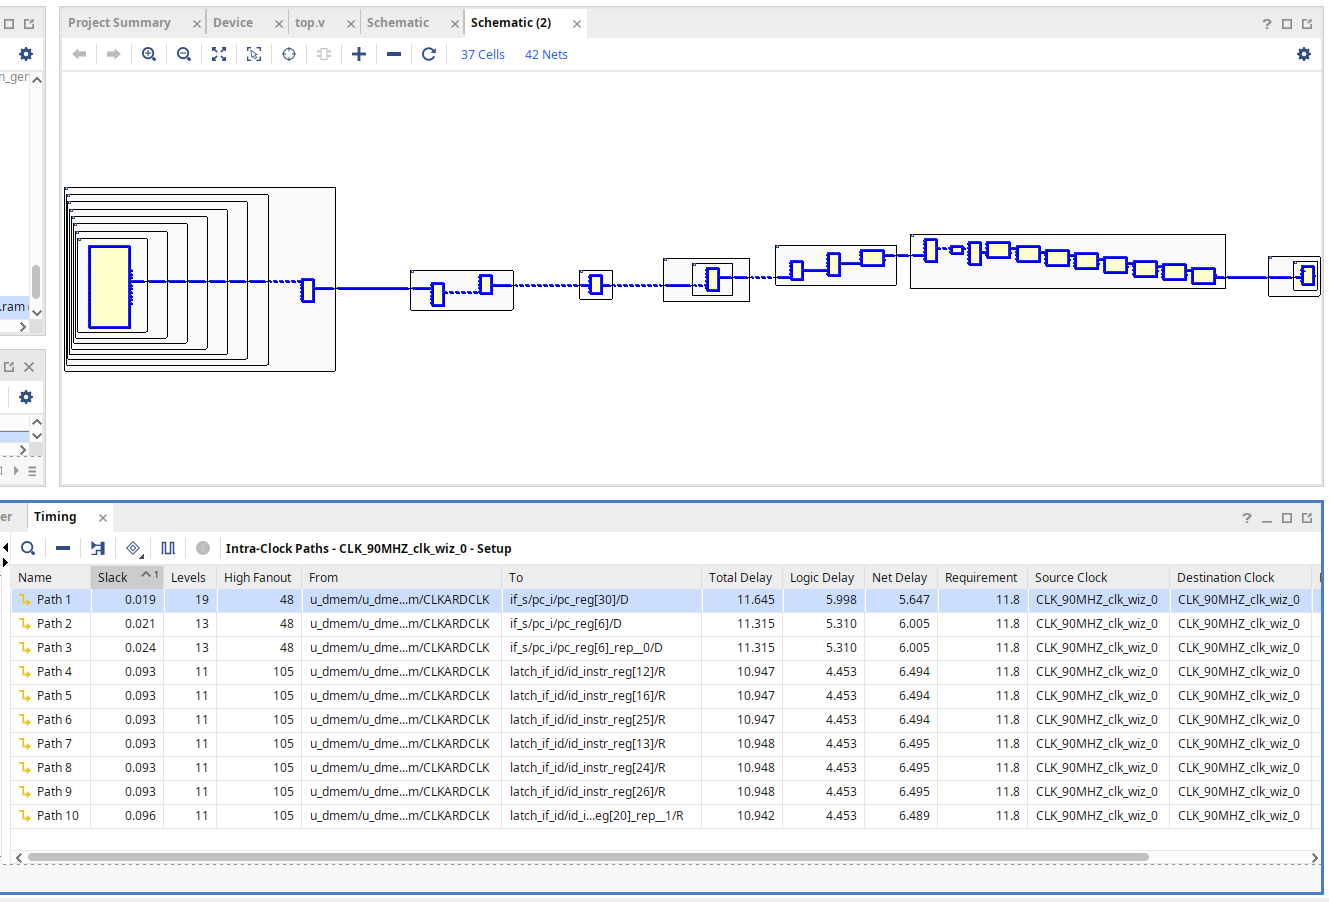
\includegraphics[width=\textwidth]{img/camino.png}
    \caption{Camino crítico identificado por Vivado, comprometiendo principalmente a las etapas MEM, WB, ID e IF del pipeline.}
    \label{fig:camino_critico}
\end{figure}

El análisis del camino crítico mostró que el retardo más exigente del sistema no se concentra en un único bloque aislado, sino en un recorrido que enlaza varias partes relevantes de la arquitectura. De acuerdo con el esquema del camino crítico reportado por Vivado, dicho recorrido parte desde la memoria de datos, atraviesa la lógica de selección del dato de escritura de la etapa de \textit{write back}, interactúa con el banco de registros y la etapa de decodificación (\texttt{regfile32}, \texttt{id\_stage}) y finalmente alcanza la lógica de actualización del contador de programa y registros vinculados a la etapa de \textit{instruction fetch} (\texttt{pc} e \texttt{if\_id\_reg}).

Desde el punto de vista arquitectónico, esto implica que en el camino crítico intervienen principalmente las etapas \textbf{MEM}, \textbf{WB}, \textbf{ID} e \textbf{IF}. En otras palabras, el dato leído desde memoria debe propagarse hasta la lógica de escritura de registros, afectar señales utilizadas durante la decodificación y participar luego en la lógica que condiciona la actualización del PC y de los registros inter-etapa. Esta extensión del recorrido explica por qué el retardo total no depende únicamente de operadores aritméticos o multiplexores, sino también de la propagación a través de varios módulos conectados entre sí.

\begin{figure}[H]
    \centering
    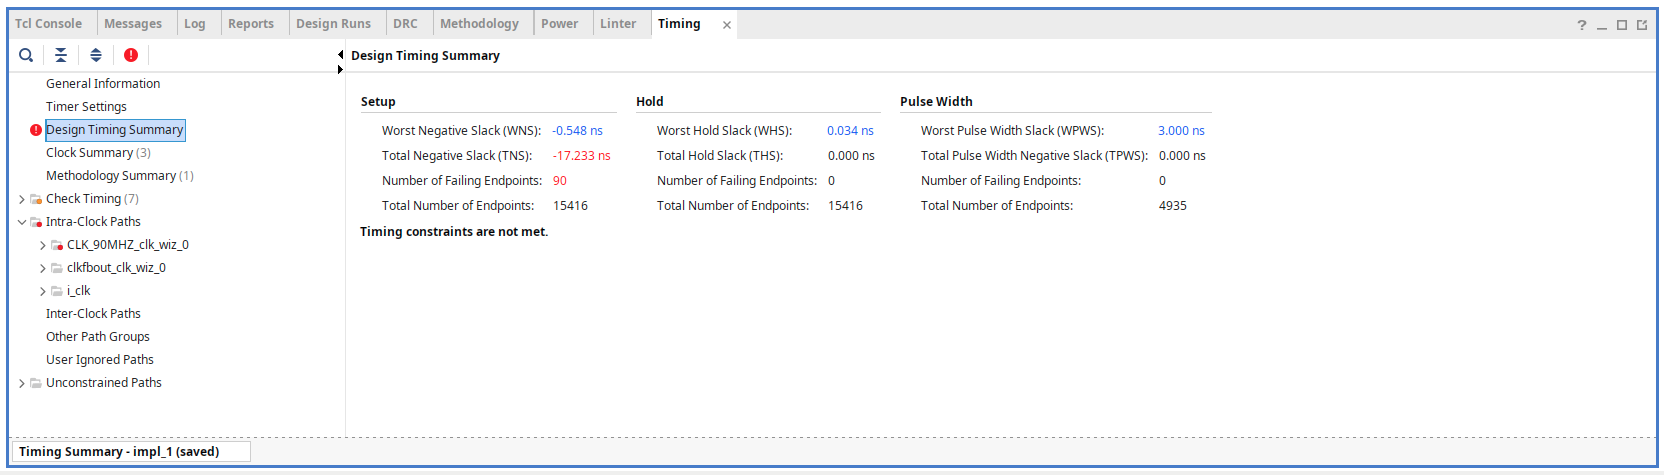
\includegraphics[width=\textwidth]{img/summary.png}
    \caption{Resumen temporal de implementación en una configuración que no alcanzaba a cumplir las restricciones impuestas. Se observa una violación de \textit{setup}, con \textit{Worst Negative Slack} negativo y múltiples endpoints en falla.}
    \label{fig:timing_summary}
\end{figure}

\begin{figure}[H]
    \centering
    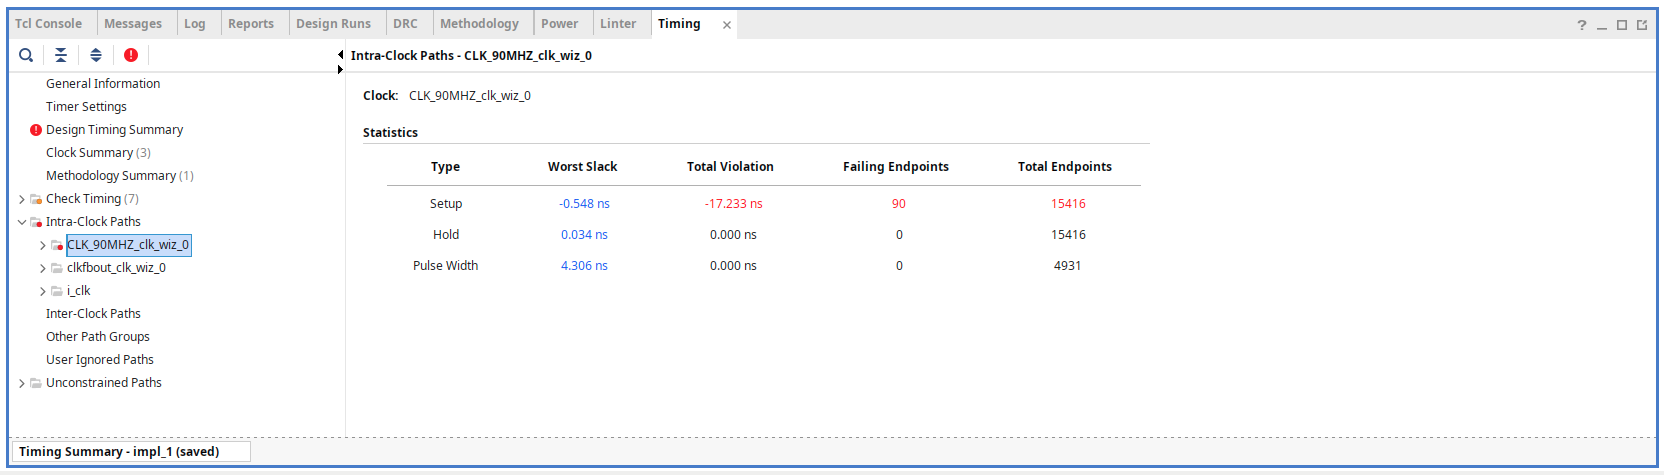
\includegraphics[width=\textwidth]{img/intra-clock.png}
    \caption{Resumen de caminos \textit{intra-clock}. Se observa que las violaciones temporales se concentraban dentro de un mismo dominio de reloj.}
    \label{fig:intra_clock_paths}
\end{figure}

Los reportes mostraron que el retardo total del camino crítico se reparte de manera comparable entre \textit{logic delay} y \textit{net delay}. Esto indica que el problema no se debe sólo a la profundidad combinacional, sino también al costo de interconexión física entre bloques, aspecto particularmente importante cuando el diseño crece en complejidad y el ruteo comienza a tener un peso similar al de la propia lógica.

\begin{figure}[H]
    \centering
    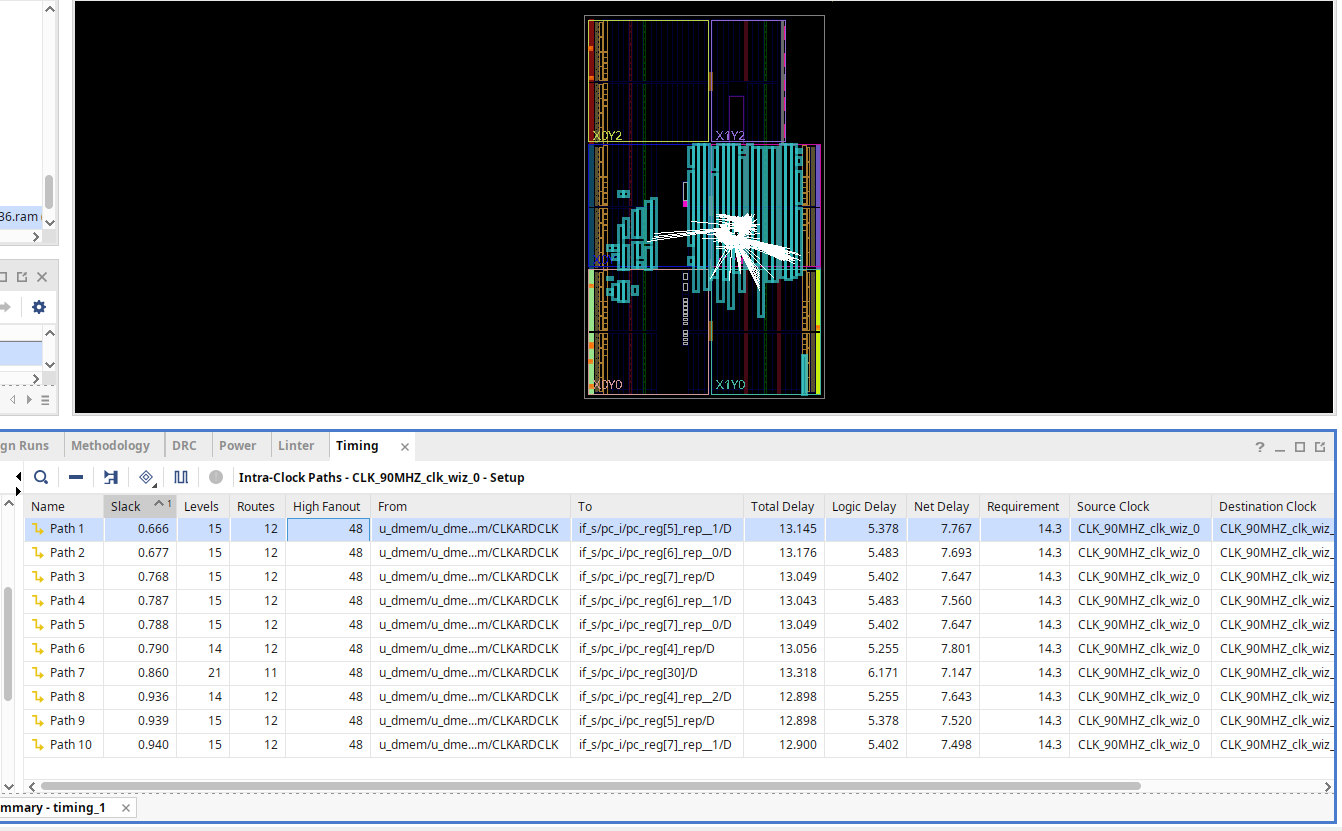
\includegraphics[width=\textwidth]{img/timing_routing.png}
    \caption{Visualización del ruteo.}
    \label{fig:timing_routing72mhz}
\end{figure}

\begin{figure}[H]
    \centering
    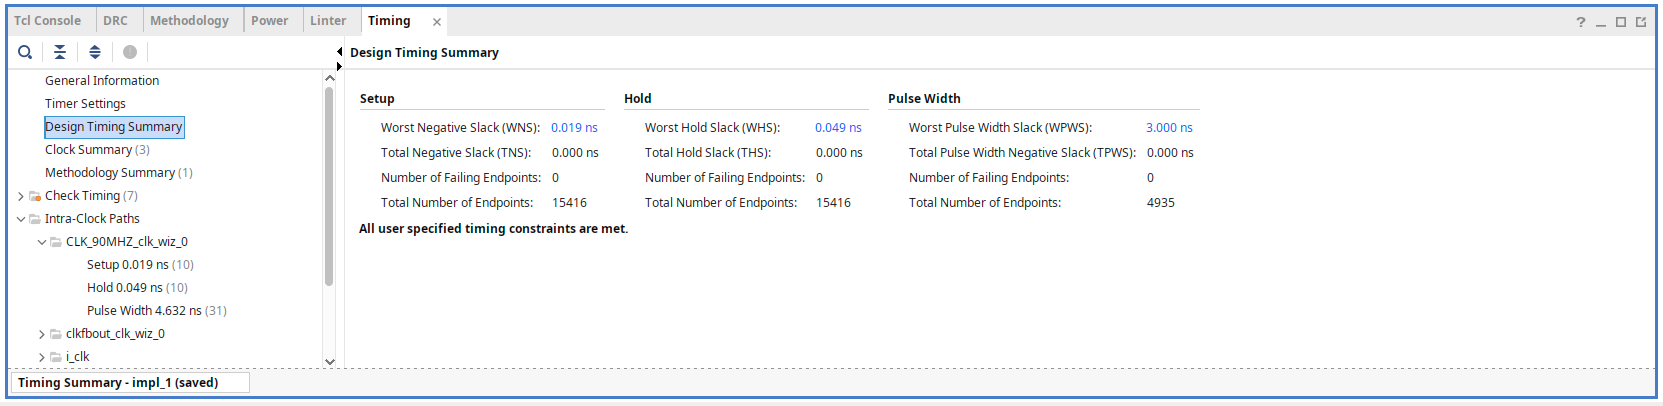
\includegraphics[width=\textwidth]{img/timing_summary.png}
    \caption{Resumen temporal de la implementación final. Se verifica que todas las restricciones temporales especificadas se cumplen, con \textit{Worst Negative Slack} positivo y sin \textit{endpoints} en falla.}
    \label{fig:timing_summary_72mhz}
\end{figure}

En este contexto, la selección final de \textbf{72 MHz} representó un compromiso razonable entre rendimiento y robustez temporal. Esta configuración permitió conservar el comportamiento correcto del pipeline, la interacción con memorias y el funcionamiento de la unidad de depuración, manteniendo un margen temporal más adecuado para la implementación completa del sistema.




% \subsection{Identificación del Camino Crítico y Skew}
% En una arquitectura segmentada, el objetivo principal del pipeline es aumentar el rendimiento permitiendo que varias instrucciones avancen en paralelo. Sin embargo, el período mínimo de reloj sigue estando condicionado por el camino combinacional más largo del diseño, es decir, por el llamado \textit{camino crítico}.

% En este trabajo, el camino crítico se encontró asociado a la interconexión entre registros del pipeline y lógica de procesamiento involucrada en la ejecución de instrucciones, particularmente en los recorridos que incluyen \textbf{cálculo de resultados, selección de datos mediante multiplexores y escritura posterior en registros}. Según la configuración sintetizada, estos caminos pueden involucrar la salida de memoria, los registros intermedios del pipeline, la lógica de selección del dato de escritura y su retorno hacia el banco de registros.

% Este resultado es coherente con la experiencia de desarrollo, ya que una parte importante de la depuración se centró precisamente en comprender cómo se propagaban los datos entre etapas y en qué ciclo exacto quedaban disponibles. La interacción entre memorias, registros de pipeline y lógica de selección resultó ser un punto especialmente sensible, tanto desde lo funcional como desde lo temporal.

% Junto con el camino crítico, también resulta relevante considerar el \textit{clock skew}, es decir, la diferencia de tiempo con la que el flanco de reloj llega a distintos registros del circuito. Aunque este efecto forma parte normal de cualquier implementación física, su influencia se vuelve más importante a medida que se exige una frecuencia de operación mayor.

% Si el margen temporal disponible es demasiado reducido, el skew puede contribuir a violaciones de \textit{setup time}, impidiendo que una señal llegue y se estabilice correctamente antes del siguiente flanco de reloj. Por eso, no alcanza con que la lógica sea funcionalmente correcta: también debe cumplir con las restricciones temporales impuestas por la tecnología y el ruteo físico sobre FPGA.

% \subsection{Determinación de la Frecuencia Óptima}
% A partir de los resultados de síntesis e implementación, se buscó determinar una frecuencia de operación que ofreciera un equilibrio entre rendimiento y robustez temporal. Para ello, se analizaron los valores de \textit{slack} obtenidos en los reportes de timing, procurando mantener un margen positivo que garantizara un funcionamiento confiable del procesador.

% Durante el desarrollo, se trabajó principalmente con relojes del orden de decenas de MHz, y se evaluó también el comportamiento del sistema frente a distintas configuraciones de frecuencia. Este análisis resultó importante no solo para validar la CPU en sí, sino también para asegurar la correcta interacción con módulos auxiliares como la UART y las memorias embebidas.

% En este contexto, se observó que no siempre la máxima frecuencia teórica resultaba ser la opción más conveniente para la validación completa del sistema. En varias etapas del proyecto fue preferible priorizar una configuración estable y repetible, que permitiera verificar correctamente la ejecución del pipeline, el intercambio UART y la depuración interna, antes que exigir el límite absoluto de operación.

% Por lo tanto, la frecuencia de trabajo adoptada se definió considerando no solo el cumplimiento de timing, sino también la estabilidad global del sistema, la reproducibilidad de las pruebas y la correcta integración entre todos los módulos del procesador.

\newpage

\section{Conclusiones}

El desarrollo de este trabajo permitió trasladar a una implementación concreta sobre FPGA varios de los conceptos centrales de arquitectura de computadoras estudiados durante la cursada. La construcción de un procesador \textit{RISC-V} segmentado en cinco etapas implicó no sólo diseñar el camino de datos y la lógica de control, sino también resolver problemas reales de integración entre módulos, temporización, manejo de riesgos y validación funcional, que exceden el análisis puramente teórico de la arquitectura.

Uno de los aspectos más relevantes del proyecto fue la incorporación de una \textit{Debug Unit} como mecanismo de control y observabilidad del sistema. Esta unidad permitió desacoplar la lógica de ejecución del procesador de las tareas de depuración, posibilitando la carga de programas por UART, la ejecución continua o paso a paso, la detención controlada y el volcado del estado interno del sistema. Contar con esta herramienta resultó fundamental para validar el comportamiento del procesador, detectar errores de manera sistemática y facilitar el análisis del tránsito de instrucciones a través del \textit{pipeline}.

Desde el punto de vista funcional, la implementación de mecanismos de \textit{forwarding}, \textit{stall} y \textit{flush} permitió resolver adecuadamente los principales riesgos asociados a una arquitectura segmentada. Las pruebas realizadas mostraron que el procesador mantiene la correctitud de ejecución frente a dependencias de datos, conflictos del tipo \textit{load-use} y cambios de flujo producidos por saltos y bifurcaciones. Del mismo modo, el tratamiento del \texttt{HALT} y el drenado del \textit{pipeline} evolucionaron hacia un esquema más robusto, basado en la detección efectiva del vaciado de los registros inter-etapa, lo que permitió garantizar una finalización consistente de la ejecución.

A lo largo del desarrollo surgieron además distintas dificultades prácticas que enriquecieron el alcance formativo del trabajo. Entre ellas se destacaron el ajuste de la latencia efectiva de las memorias para alinearla con lo esperado por el \textit{pipeline}, la diferenciación conceptual entre pausa externa y terminación interna, y la validación del protocolo UART en escenarios de comunicación más extensos, como los volcados de registros, latches y memoria. La resolución de estos problemas llevó a un diseño más claro, modular y coherente, y obligó a adoptar criterios de validación más precisos tanto en simulación como en hardware real.

En conjunto, los resultados obtenidos indican que el sistema desarrollado cumple con los objetivos propuestos y constituye una implementación sólida y funcional del procesador requerido. Más allá del cumplimiento del trabajo práctico, el proyecto integró conocimientos de diseño digital, arquitectura de computadoras, verificación, temporización e interacción entre hardware y software, ofreciendo una experiencia de desarrollo completa sobre FPGA.

\end{document}
